
\chapter{Software fundamentals}



\important{
IMPORTANT NOTE: this manual is still under development! For the moment, it is still far from complete and only gives a very brief description of the most important aspects of the software.
}




\section{General concepts}

\softwarename\ is almost entirely script driven. Scripts are text files with the extension \filename{.sci}, and contain source code written in a special, simple but powerful rendering language, called \scriptlang. The software comes with a number of ready--to--use sample scripts, but you are free to write your own script, or adapt the existing ones. An introduction on programming in \scriptlang\ can be found in chapter \ref{scriptdevelopment}.

Everything in the software is driven by a script: the animations itself, but also the startup screen and the tool for changing the settings. \softwarename\ comes with a set of pre--defined scripts, but nothing prevents you from modifying these scripts, and overrule the default behaviour. In this way, \softwarename\ can be completely adapted to your desires.

The software has two types of windows, the \sourcewin\ and the \renderwin. There is always exactly one \sourcewin\ present when the software starts, and this window is used for the development and testing of animation scripts. During an animation, this window is not visible.

There can be zero, one or more \renderwins, depending on the current state of the software. These are the windows where the actual renderings are visualised. Typically, there will be one \renderwin\ that fills the entire display of the computer, and the \sourcewin\ is obscured behind this \renderwin. Should you want to pop op the \sourcewin\ in order to start editing scripts, you can activate it with the standard Windows tools (such as the Alt+TAB keyboard combination).

\section{Data organisation and settings}

Settings in \softwarename\ are specified in the scripts. There is only one setting that is optionally is stored in the registry: the \datadir\ where \softwarename\ looks for its data. This directory is stored in the registry in \filename{HKEY CURRENT USER/Software/Z-Flux/Z-Flux/Settings/DataDirectory}. It can also be set in the settings dialog box, accessible from the  \sourcewin. If no \datadir\ is specified in the registry, the software looks in the default location, which is the "Data" subdirectory of the folder where the executable was started from.


The \datadir\ contains a large amount of data files that are crucial for the correct functioning of the software. These files are organised into a number of subdirectories. It also contains a subdirectory ``Scripts'', where all the animation scripts are stored. Note that \softwarename\ should have read and write privileges on this directory, without the need to become an administrator. This is particularly important for Windows Vista or Windows 7, because the Program Files directory is read--only for a normal user. On these operating  systems, you should make sure that the \datadir\ is not under this directory.

Each time the software starts, it looks for a script called \filename{\_init.sci} in the ``Scripts'' subdirectory of the \datadir\ and executes it automatically. This script is responsible for the initialisation and configuration of the rendering window. 

After completion of the script \filename{\_init.sci}, the software automatically looks in the same location for a second script called  \filename{\_autorun.sci}. This script is be used to automatically start an animation. The default implementation of \filename{\_autorun.sci} is to start the pre--installed animation script \filename{\_menu.sci}, which shows a menu on the screen that allows the user to navigate through all the animation scripts that are currently present, and start them.

\section{The default startup script}

A pre--installed startup script \filename{\_autorun.sci} is provided with the installation. This script creates a menu that allows the user to browse through all animations in the ``Scripts'' subdirectory of the \datadir, and start any of these. You can browse through the top level menu item with the Up and Down arrow keys. Menu items that corresponds with subfolders can be activated by pressing the Right arrow key. Exiting such a submenu is done by pressing the Left arrow Key. To start a navigation, navigate the cursor to it and press the Enter key. You can stop the animation by pressing the Escape key, and the startup menu will be shown again.

\section{The Settings script \label{settings}}
An important pre--installed script is the ``Settings'' script, which can be accessed from the main menu. Here you can customise several important aspects of the way the animations are rendered. You can navigate through the controls on the display using the TAB key or the Left/Right arrow keys, and change the status of a congtrol using the Up/Down arrow keys and the Enter key. To validate the changes, navigate to the "Apply" button and press Enter. Below is a list of all controls that are present in the Settings view:
\begin{description}
\item[Show in stereo] Determines whether the animations are rendered in monoscopic mode (i.e. a single view), or in stereoscopic mode (i.e. two side--by--side images for the left and the right eye). See \ref{stereorendering} for more information about stereo rendering.
\item[Swap left and right] If stereo rendering is active, this option will reverse the ordering of both image (Left eye--Right eye or Right Eye--Left eye).
\item[Left mirror horizontal] Mirrors the image of the left eye horizontally. Note that, if stereo rendering is disabled, the single image that is displayed is called the left eye image.
\item[Right mirror horizontal] Same for the right eye image.
\item[Left mirror vertical]. Mirrors the image vor the left eye vertically.
\item[Right mirror vertical]. Same for the right eye. All four mirror options, together with the Left--Right swapping option, allow the user to tune the software for virtually every stereo rendering system where both images are shown side by side.
\item[Horizontal Stretch] Sets a stretch of compression factor for the image in the horizontal direction. This can be useful to obtain a correct image in case the animations are rendered to a device that has non-rectangular pixels.
\item[Eye separation factor] This is an important setting in case stereo rendering is used. See \ref{stereobaseline} for more information about this value.
\item[Display name] Can be left empty in most cases.
\item[Full screen] This option determines if the rendering window runs in "Full Screen" mode.
\item[Display offset X] The horizontal offset in pixels of the rendering window, measured from the left edge of the display.
\item[Display size X] The horizontal size of the rendering window in pixels.
\item[Display offset Y] The vertical offset in pixels of the rendering window, measured from the top of the display.
\item[Display size Y] The vertical size of the rendering window in pixels.
\item[Frame rate] The number of frames that should be rendered per second. Note that this is only a target number: if the hardware is too slow to render a given animation at this speed, it will automatically slow down. For optimal results, this value should be equal to the refresh rate of the display, or an integer fraction of it (e.g. 60, 30, 20, 15... if the refresh rate is 60Hz).
\item[Sync factor] Determines how many refresh cycles are skipped between each rendering action. This option can also be used as an alternative way to set the frame rate (a sync factor of 2 on a system with a refresh rate of 60Hz will result in a frame rate of 30)
\item[Language] Sets the language to which the text in the animations will be translated.
\item[Apply] Applies the current settings. The software will have to be restarted.
\item[Cancel] Cancels the changes performed and returns to the startup script.
\end{description}

\important{When changes are applied by pressing the \term{Apply} button, \softwarename\ will automatically close, and you will have to restart to run the software with the new settings. However, some combinations of settings are not compatible with all hardware and software. In such a case, \softwarename\ will fail to load with the new configuration. You can solve this by editing the file \filename{settings.txt} in the \datadir. The easiest solution is to remove all content of this file completely, which will cause \softwarename\ to revert to the default settings. Alternatively, you can edit the settings parameters directly in this file.
}

\section{Sample animations}
\softwarename\ comes with a set of pre--defined animations. In the current version, this set is far from complete and only serves as a limited showcase for what is possible with this software. These scripts can also serve as a basis for writing your own animations. From the menu created by the startup script, you can browse through the animations with the cursor keys, and start a particular one with the Enter key. To exit this animation and return to the start menu, press Escape.


\section{Stereo rendering \label{stereorendering}}
\softwarename\ can render the animations to a traditional computer monitor, creating a 2D monoscopic image of the 3D content. But, more important, on the appropriate hardware, it can also render scenes in 3D by creating stereoscopic images (see \ref{settings} on how to enable stereo rendering). To this end, each frame is rendered two times, one time for the left eye and one time for the right eye. Both renderings are shown side by side on the \renderwin\ (\figref{stereosample}).

\begin{figure}
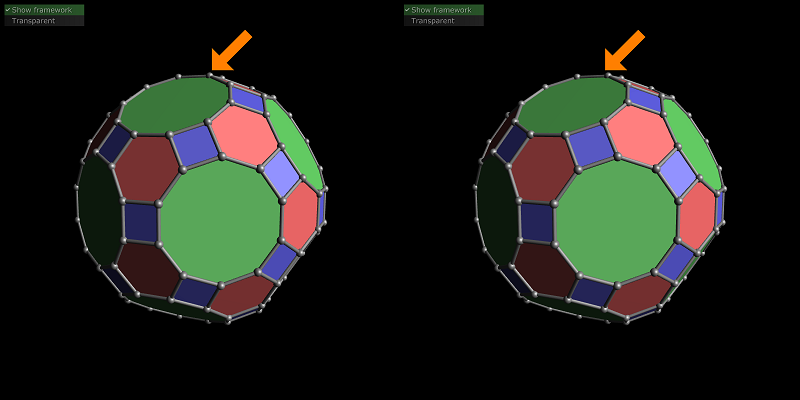
\includegraphics[scale=0.4]{bitmaps/stereosample.png}
\caption{A sample stereo rendering of a polyhedron with a cursor on top.}
\label{stereosample}
\end{figure}


\subsection{Polarisation stereo projection}
One of the principal aims of \softwarename\ is to work in conjunction with stereo projection systems that are based on polarisation. Such polarisation stereo projection systems (also sometimes called passive stereo) offer high quality immersive 3D projection at a low cost, and  typically consist in the following relatively items:
\begin{itemize}
\item A computer with a fast graphics card and dual screen output, running appropriate software (such as \softwarename).
\item Two data projectors that are connected to both screen outputs.
\item Two different polarising filters that are fitted in front of the projectors (e.g. 45� left and 45� right)
\item A non--depolarising projection screen (sometimes also called a silverscreen)
\item A number of polarised looking glasses.
\end{itemize}
See e.g. the GeoWall consortium (\url{http://www.geowall.org/} or \url{http://en.wikipedia.org/wiki/GeoWall}) for more information about how this kind of stereo visualisation systems work, and how to assemble such a system.

In order to configure \softwarename\ to work properly on such a system, it is crucial to realise that the left eye image should be sent to one projector, and the right eye image to the other. This can be achieved using the dual monitor feature of Windows, which creates a single virtual desktop that spans over both projectors. The \renderwin\ used \softwarename\ should then be configured in such a way that is exactly spans over the full desktop, and hence covers both screens. The left half of the \renderwin\ will then be sent to the left projector, and the right half to the right projector. Since, in stereo mode, \softwarename\ displays the left eye rendering and the right eye rendering side by side, the desired setup should be achieved.

You can setup the dimensions of the \renderwin in the settings scripts (see \ref{settings}). More specifically, \textbf{Display offset X} and \textbf{Display offset Y} specify the position of the top left corner of this window, in pixels, whereas \textbf{Display size X} and \textbf{Display size Y} specify the horizontal and vertical dimension of the \renderwin, also in pixels.

For example, suppose that two projectors are used with a resolution of $1024 \times 768$ pixels. The dual screen modus of Windows will create a single, virtual desktop that puts both projectors side by side, creating a total desktop resolution of $2048 \times 768$ pixels. In order to make \softwarename\ work correctly on such a system, the following values should be entered:

\begin{tabular}{l l}
\hline
Setting & Value \\ \hline
Show in stereo & checked \\
Swap left and right & \textit{dependent on the cabling of the projectors} \\
Display offset X & 0 \\
Display offset Y & 0 \\
Display size X & 2048 \\
Display size Y & 768 \\
\hline
\end{tabular}

\subsection{Parallel viewing and cross viewing}
A low budget way of viewing the animations in 3D is by simply looking at them side by side on a computer monitor, and try to make the stereo effect pop up. You can set up the image size that is optimal for this kind of viewing on your system by changing \textbf{Display Size X} and \textbf{Display Size Y}.

\subsection{Mirror viewing}
Another great way to see the animations in stereo is the usage of mirrors or prisms (see e.g. 
\url{http://nzphoto.tripod.com/sterea/stereomirror.htm}). To facilitate this kind of viewing, \softwarename\ offers complete freedom when it comes to flipping both stereo images. For both the left and right eye image, you can independently chose to mirror the image horizontally and/or vertically.

\subsection{The stereo baseline and stereo distance \label{stereobaseline}}
Two important parameters determine the way a scene is visualised in stereo:
\begin{description}
\item[Stereo distance] When a 3D scene is visualised as a stereo pair on a device (e.g. projected on a screen using polarisation projection), the viewer will see each component of the scene at a specific distance with respect to the screen. Some components will appear to float in front of the screen (hence this is often called immersive 3D), other components will appear to be at the same distance of the screen, and other components will appear behind the screen. Objects that appear at the same distance of the screen are said to have a zero parallax, because they have exactly the same position on both eye images. The stereo distance is the distance, measured in the 3D scene, from the viewer at which components of the scene are rendered with zero parallax.
\item[Stereo baseline] This is the distance between the left and right eye camera position in the scene. In many cases, it is meaningless to render a scene with a stereo baseline that is identical to the distance between the human eyes. For example, suppose that the animation shows the movement of the Planets around the Sun. A ``normal'' stereo baseline would show all planets at a distance of infinity, just like we see the stars in reality. Of course, in that case, the advantage of using a 3D rendering vanishes. Therefore, it is customary to use ``hyperstereo'', a technique where the stereo baseline is artificially boosted. The effect of hyperstereo can be interpreted in two ways:
\begin{enumerate}
\item A huge creature, with a large distance between both eyes, looks at the scene.
\item A normal human being (with standard eye separation) looks at a reduced scale model of the scene. The reduction factor is equal to the magnification factor of the stereo baseline.
\end{enumerate}
\end{description}
Most animations in \softwarename\ automatically control the stereo distance in a meaningful way, depending on the scene that is shown. In addition, the stereo baseline is automatically set as a constant fraction of the stereo distance, which ensures that a reasonable 3D effect is always visible. This fraction is determined by the \textbf{Eye separation factor} parameter in the settings.



\section{Warped rendering}
With\softwarename, it is possible to apply a two-dimensional distortion to the rendered image. This can be useful in a number of different situations, e.g.:
\begin{itemize}
\item Dome projection using a fisheye lens or a spherical mirror
\item Visualisation of 360-degree stereo pictures
\item Special projections, e.g. making a celestial chart
\end{itemize}

The definition of the warping can be specified in the init script. Below is an example of how this can be implemented:

\begin{lstlisting}
vp=addviewport(0,0,1,1,displayname,displayname);
...
warpx=matrix(101,101);
warpy=matrix(101,101);
for ix=0 to 100 do
   for iy=0 to 100 do {
      x=ix/100;
      y=iy/100;
      warpx(ix,iy)=x/(1+y);
      warpy(ix,iy)=y*(0.5+0.5*x);
   }
vp.EnableWarped(2000,1500,warpx,warpy);
\end{lstlisting}
